%% LaTeX2e class for student theses
%% sections/content.tex
%% 
%% Karlsruhe Institute of Technology
%% Institute for Program Structures and Data Organization
%% Chair for Software Design and Quality (SDQ)
%%
%% Dr.-Ing. Erik Burger
%% burger@kit.edu
%%
%% Version 1.3.3, 2018-04-17

\chapter{Related Work}
\label{ch:RelatedWork}
With the exponentially increasing amount of acquired multivariate data, several multi-dimensional visualization techniques have been proposed during the last decades. Parallel coordinates and scatterplot matrices are widely used to visualize multi-dimensional data sets. But these visualization techniques are insufficient when the number of dimensions grows. To solve this problem, different approaches to select the best views or dimensions in advance have been proposed in the last years.\\ 
\begin{figure}[h]
	\centering
	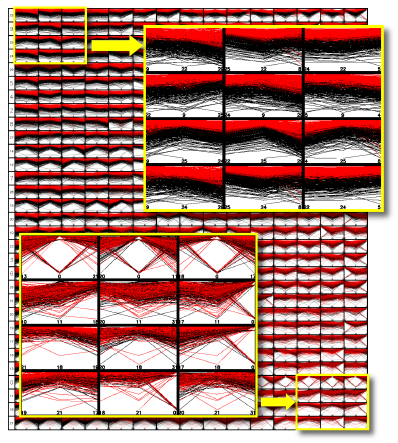
\includegraphics[width=0.4\textwidth]{pictures/PCM}
	\caption{Parallel coordinates matrices\cite{Matrics} for the data set}
	\label{fig:PCM}
\end{figure}
\\Georgia Albuquerque et al. presented three new methods to explore multivariate data sets: a parallel coordinates matrix (\autoref{fig:PCM}), in analogy to the well-known scatterplot matrix, a class-based scatterplot matrix that aims at finding good projections for each class pair (\autoref{fig:C-SPLOM}), and an importance aware algorithm\cite{Matrics} to sort the dimensions of scatterplot and parallel coordinates matrices. They aims at providing a visualization of the whole data set, not the correlations of attributes in this data set. As we focus on the correlations only between each two attributes in our thesis, it is no need for us to have parallel coordinates in our framework.
\begin{figure}[h]
	\centering
	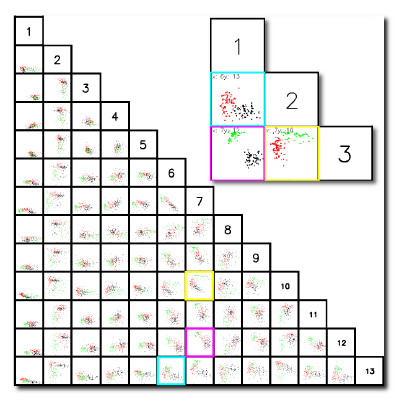
\includegraphics[width=0.4\textwidth]{pictures/C-SPLOM}
	\caption{Class-based scatterplot matrices\cite{Matrics} for the data set}
	\label{fig:C-SPLOM}
\end{figure}
\\In \autoref{sec:Introduction:Motivation}, we have pointed out the use and importance of correlation analysis between different attributes, which helps people to understand the relationship of attributes in a data set. Unlike the work of Georgia Albuquerque et al.\cite{Matrics}, our interface provides the visualization of correlation values in a data set.\\
As a high-dimensional data set may contain many redundant features, feature selection becomes an essential step for correlation analysis. Louis Kirsch et al. developed an interactive Framework for Exploring and Understanding Multivariate Correlations (FEXUM)\cite{FEXUM} to simultaneously visualize all feature correlations to the target and pairwise correlations using Force-Directed-Graph. This visualization provides a layout in which a smaller distance between two features denotes a greater redundancy. In \autoref{fig:FEXUM}, nodes represent features and weighted edges represent distances. FEXUM provides users with an understanding of how features interact with each other in terms of redundancy so that they can easily find influential value ranges in the analysis view and make feature selection.\\
In our developed interface, we give the users an overview of all correlations in the data set. Instead of choosing a target attribute to focus on, our system represents the whole correlations of the data set. Unlike FEXUM\cite{FEXUM}, Force-Directed-Graph is not the only visualization method in our system. Heat map and Bar graphs are alternative visualization method for the users so that the users can choose the most suitable visualization method in their opinion.\\
In \autoref{sec:Introduction:Challenges:Streams}, we have discussed that the correlation analysis should be a continuous process. FEXUM enables the users to upload their own data sets and visualize them. However, in our system, the uploaded data set by users can be a data set of data stream so that the users can choose a period of time to perform the correlation analysis and visualization. Our goal is to visualize a concise but useful summary of correlations in the stream over time.\\
\begin{figure}[h]
	\centering
	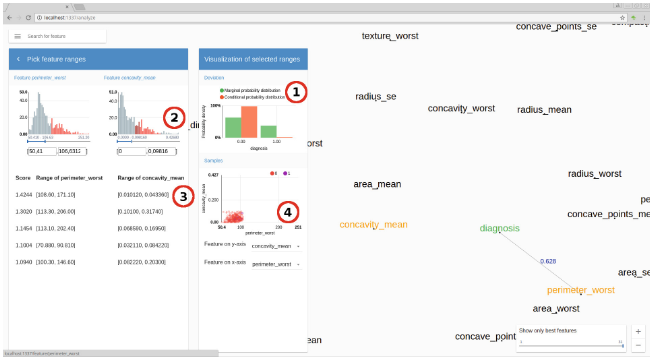
\includegraphics[width=\textwidth]{pictures/FEXUM}
	\caption{Features drawn using a force-directed graph (right), with the target highlighted in green. An analysis view of two features (left) for inspecting the correlations.\cite{FEXUM}}
	\label{fig:FEXUM}
\end{figure}